\newpage
{\bfseries МРНТИ 27.47.19}
\hfill {\bfseries \href{https://doi.org/10.58805/kazutb.v.3.24-509}{https://doi.org/10.58805/kazutb.v.3.24-509}}

\sectionwithauthors{Б.Б. Оразбаев, Л.Т. Салыбек, Л.Т. Курмангазиева, В.И. Терехов, Б.Е. Утенова, В.Е. Махатова, А.С.Өтебаева}{МҰНАЙДЫ БАСТАПҚЫ ӨҢДЕУ ҚОНДЫРҒЫСЫНДА ТҰРАҚТЫ БЕНЗИН ӨНДІРУ ПРОЦЕСІН АЙҚЫНСЫЗДЫҚТА МОДЕЛЬДЕРІ НЕГІЗІНДЕ ОҢТАЙЛАНДЫРУ ТӘСІЛІ}

\begin{center}
{\bfseries \textsuperscript{1}Б.Б. Оразбаев, \textsuperscript{2}Л.Т.
Салыбек\textsuperscript{🖂}, \textsuperscript{3}Л.Т. Курмангазиева,
\textsuperscript{4}В.И. Терехов, \textsuperscript{5}Б.Е. Утенова, \textsuperscript{3}В.Е. Махатова, \textsuperscript{3}А.С.
Өтебаева}

\textsuperscript{1} Л.Н. Гумилев атындағы Еуразия ұлттық университеті,
Астана, Қазақстан,

\textsuperscript{2} М.О. Әуезов атындағы Оңтүстік Қазақстан
университеті, Шымкент, Қазақстан,

\textsuperscript{3} Х. Досмухамедов атындағы Атырау университеті,
Атырау, Қазақстан,

\textsuperscript{4} Н.Э. Бауман атындағы Мәскеу мемлекеттік техникалық
университеті, Москва, Ресей,

\emph{{\bfseries \textsuperscript{5}}} С. Утебаев атындағы Атырау мұнай
және газ университеті, Атырау, Қазақстан

{\bfseries \textsuperscript{🖂}}Корреспондент-автор: lyaklai.36972@mail.ru \vspace{0.5cm}

\end{center}
Бұл мақалада мұнайды бастапқы өңдеу қондырғысының мақсаттық өнімі болып
табылатын тұрақты бензин өндіру процесін оның математикалық негіздері
негізінде айқынсыздық жағдайында оңтайландыру мәселелері зерттеліп,
оларды тиімді шешу әдістемелері ұсынылған. Қазіргі уақытта мұнай өңдеу
өндірісінде мұнайды бастапқы өңдеу қондырғысында өтетін негізгі
процесстердің оңтайланландыру есебін шешу алынған мұнай өнімдерін ары
қарай терең өңдеу процесстері тиімділігін қамтамасыз ететіндіктен аса
өзекті ғылыми, өндірістік мәселенің біріне жатады. Осыған байланысты бұл
зерттеуде Атырау мұнай өңдеу зауытының мұнайды бастапқы өңдеу
қондырғысының мақсатты өнімі − тұрақты бензин өндіру процесін ондағы
айқынсыздық жағдайында оңтайландыру есебі математикалық тұжырымдалып,
оны айқын емес ортада тиімді шешу үшін эвристикалдық тәсілдеме
ұсынылған.

Орындалған зерттеулер нәтижесінде мұнайды бастапқы өңдеу қондырғысының
тұрақтандыру колоннасы сияқты кей параметрлері айқынсыздықпен
сипатталатын күрделі нысандардың математикалық модельдерін құрып,
олардың негізінде нысанның айқынсыздықта жұмыс режимін тиімді
оңтайландыратын эвристикалық тәсілдеме әзірленген. Тұрақтандыру
колоннасынан алынатын тұрақты бензин мен газ көлемдерін колоннаның
кіріс, режимдік параметрлерне байланыста анықтайтын модельдер
регрессорларды тізбектей қосу тәсілдемесі мен ең кіші квадраттар тәсілін
жүйелі қолдану арқылы, экспертменталдық-статитстикалық деректер
негізінде идентификацияланған. Ал тұрақты бензинің айқынсыздықпен
сипатталатын сапа көрсеткіштерін бағалайтын айқын емес модельдер
эксперттік бағалау, айқын емес жиындар тәсілдері арқылы
модификацияланған регрессорларды тізбектей қосу мен ең кіші квадраттар
тәсілдері негізінде құрылған. Алынған тұрақтандыру колоннасы модельдері
негізінде тұрақты бензин өндіру процесін айқынсыздықта тиімді
оңтайландыру үшін әзірленген эвристикалық алгоритм Парето оптималдық пен
идеалды нүкте оптималдық принциптері мен олардың комбанациясын
айқынсыздыққа модификациялауға негізделген.

{\bfseries Түйін сөздер}: көпкритерийлі оңтайландыру, айқын емес ақпарат,
айқын емес модель, айқынсыздықта шешім қабылдау, мұнайды бастпқы өңдеу
қондырғысы, тұрақтыв бензин.

\begin{center}
{\bfseries METHOD FOR OPTIMIZATION OF THE PRODUCTION PROCESS OF STABLE GASOLINE AT PRIMARY OIL PROCESSING UNITS IN A FUZZY ENVIRONMENT BASED ON OBJECT MODELS}

{\bfseries \textsuperscript{1}B. Orazbayev, \textsuperscript{2}L.
Salybek\textsuperscript{🖂}, \textsuperscript{3}L. Kurmangaziyeva,
\textsuperscript{4}V.Terekhov, \textsuperscript{5}B.Utenova, {3}V.E. Makhatova, \textsuperscript{3}A.
Otebayeva}

\textsuperscript{1} L.N. Gumilyov Eurasian National University, Astana,
Kazakhstan,

\textsuperscript{2} M. Auezov South Kazakhstan University, Shymkent,
Kazakhstan\emph{{\bfseries ,}}

\textsuperscript{3} Kh. Dosmukhamedov Atyrau University, Atyrau
Kazakhstan,

\textsuperscript{4} N. Bauman Moscow State Technical University, Moscow,
Russian,

\textsuperscript{5} S Utebaev Atyrau Oil and Gas University, Atyrau,
Kazakhstan,

e-mail: lyaklai.36972@mail.ru
\end{center}

This article examines the problems of optimizing the production process
of stable gasoline based on models of the object, which is the target
product of a primary oil refining installation, and proposes approaches
to their effective solution. Currently, solving the problem of
optimizing the main processes at a primary oil processing plant in the
oil refining industry is one of the most pressing scientific and
production problems, as it ensures the efficiency of further deep
processing of the resulting petroleum products. In this regard, this
study formulates a mathematical formulation of the problem of optimizing
the production process of stable gasoline - the target product of the
primary oil refining installation of the Atyrau Oil Refinery,
characterized by uncertainty, and proposes a heuristic approach for its
effective solution in a fuzzy environment.

As a result of the research, mathematical models of complex objects
characterized by ambiguity of some parameters, such as the stabilization
column of a primary oil treatment plant, were developed, and on their
basis a heuristic approach was developed that effectively optimizes the
operation of the object in conditions of uncertainty. Models that
determine the volumes of gasoline and gas from the stabilization column
depending on the input operating parameters of the column are determined
on the basis of experimental statistical data and the systematic
application of the approach of sequential sequential connection of
regressors and the least squares method. Fuzzy models that evaluate
vaguely described quality indicators of stable gasoline are synthesized
on the basis of expert assessment methods, fuzzy sets and modified
methods of sequential inclusion of regressors, least squares. Based on
the obtained models of the stabilization column, a heuristic algorithm
has been developed for the effective optimization of the production
process of stable gasoline under conditions of fuzzy conditions, based
on a modification and combination of the principles of Pareto optimality
and the ideal point for working in a fuzzy environment.

{\bfseries Keywords}: multicriteria optimization, fuzzy information, fuzzy
model, decision making in a fuzzy environment, primary oil refining
unit, stable gasoline.

\begin{center}

{\bfseries МЕТОД ОПТИМИЗАЦИИ ПРОЦЕССА ПРОИЗВОДСТВА СТАБИЛЬНОГО БЕНЗИНА НА УСТАНОВКАХ ПЕРВИЧНОЙ ПЕРЕРАБОТКИ НЕФТИ В НЕЧЕТКОЙ СРЕДЕ НА ОСНОВЕ МОДЕЛЕЙ ОБЪЕКТА}

{\bfseries \textsuperscript{1}Б.Б. Оразбаев, \textsuperscript{2}Л.Т.
Салыбек\textsuperscript{🖂} , \textsuperscript{3}Л.Т.Курмангазиева,
\textsuperscript{4}В.И. Терехов, \textsuperscript{5}Б.Е.Утенова, {3}В.Е. Махатова, \textsuperscript{3}А.С.
Отебаева}

\textsuperscript{1} Евразийский национальный университет имени Л.Н.
Гумилева, Астана, Казахстан,

\textsuperscript{2} Южно-Казахстанский университет имени М.О. Ауезова,
Шымкент, Казахстан,

\textsuperscript{3} Атырауский университет имени Х. Досмухамедова,
Атырау, Казахстан,

\textsuperscript{4} Московский государственный технический университет
имни Н.Э. Баумана, Москва, Россия,

\emph{{\bfseries \textsuperscript{5}}} Атырауский университет нефт и газа
имени С. Утебаева, Атырау, Казахстан,

e-mail: lyaklai.36972@mail.ru
\end{center}

В данной статье исследованы проблемы оптимизации процесса производства
стабильного бензина на основе моделей объекта, который является целевым
продуктом установки первичной переработки нефти и предложены подходы к
их эффективного решения. В настоящее время решение задачи оптимизации
основных процессов на установке первичной переработки нефти в
нефтеперерабатывающей промышленности является одной из наиболее
актуальных научных и производственных задач, так как обеспечивает
эффективность дальнейшей глубокой переработки получаемых нефтепродуктов.
В этой связи в данном исследовании сформулирована математическая
постановка задачи оптимизации процесса производства стабильного бензина
-- целевого продукта установки первичной переработки нефти Атырауского
НПЗ, характеризующиеся с нечекткостью и предложен эвристический подход
для ее эффективного решения в нечеткой среде

В результате проведенных исследований разработаны математические модели
сложных объектов, характеризующимися неоднозначностью некоторых
параметров, таких как колонна стабилизации установки первичной
подготовки нефти, и на их основе разработан эвристический подход,
эффективно оптимизирующий работу объекта в условиях нечеткости. Модели,
определяющие объемы бензина и газа из стабилизационной колонны в
зависимости от входных режимных параметров колонны, определены на основе
эксперментально-статистических данных и системного применения подхода
последовательного последовательного соединения регрессоров и метода
наименьших квадратов. А нечеткие модели, оценивающие нечетко описываемых
качественных показателей стабильного бензина синтезированы на основе
методов экспертных оценок, нечетких множеств и модифицированных методов
последовательного включения регрессоров, наименьших квадратов. На основе
полученных моделей стабилизационной колонны разработан эвристический
алгоритм эффективной оптимизации процесса производства стабильного
бензина в условиях нечеткости, основанный на модификации и комбинации
принципов оптимальности Парето-оптимальности и идеальной точки для
работы в нечеткой среде.

{\bfseries Ключевые слова}: многокритериальная оптимизация, нечеткая
информация, нечеткая модель, принятие решений в нечеткой среде,
установка первичной переработки нефти, стабильный бензин.

{\bfseries Кіріспе.} Бүгінгі таңда әлем, соның ішінде Қазақстан
экономикасында мұнай өңдеу өндірісінде мұнайды бастапқы өңдеу
процесстері мен оларды оңттайландыру, тиімді басқару мәселелері аса
маңызды да, өзекті мәселелердің бірі болып табылады. Оның негізгі
себептері ретінде:

− әр салаға өте қажетті сапалы мұнай өнімдерін алудың шикі мұнайды су,
тұздан тазарту мен алғашқы өңдеу сапасының маңыздылығын;

− мұнайды бастапқы өңдеу процесінде ауыр мұнай өнімдері фракциялары
есебінен, негізгі мақсаттық өнімі болып табылатын бензиннің жеңіл
фракцияларын − тұрақты бензинді қажетті сапасын қамтамасыз ете отырып,
барынша арттырудың аса қажеттігін атап өтуге болады {[}1-3{]}.

Шикі мұнайды су, тұз және түрлі мехапникалық қоспалардын тазартатын және
тазарған мұнайды бастапқы өңдеу процесстері барлық мұнай өңдеу
зауыттарындв (МӨЗ) бар мұнайды бастапқы өңдеу қондырғыларында (МБӨ)
өтеді. Бұл МБӨ қондырғылары басқа да технологиялық қондырғылар сияқты өз
ара материалдық, энергиялық, ақпараттық ағындармен байланысты көптеген
технологиялық агрегаттардан тұратын күрделі технологиялық жүйелерге
жатады.

Мұндай технологиялық жүйелердің жұмыс сапасы әдетте экономикалық,
экологиялық, технологиялық сипаттағы көптеген критериицлермен бағалады
{[}4,5{]}. Сонымен қатар МӨЗ-да қолданыстағы МБӨ қондырғылдарында
өндірілетін мұнай өнімдерінің түрлі фракциялары (ауыр, жеңіл, керосин,
мазут) фракцияларының сапасы көрсеткіштері практикада адам, яғни
мамандар қатысуымен, олардың білімі, тәжірибесі, яғни айқын емес
ақпараттар негізінде лабораториялық жолмен бағалады {[}6 - 8{]}. Оған
қасымша қолданыстағы стандарттар талваптары бойынша бензин, басқа да
мұнай өнімдерінің қайнау температуралы, құрамы сияқты сапа көрсеткіштері
«көп емес», «аз емес», берілген міннен «артық» не «кем» сияқты айқын
емес нұсқаулермен сипатталады {[}9, 10{]}.

Жоғарыда сипатталған МБҚ қондырғысының практикадағы айқынсыздықпен
сипатталауы және оның жұмыс сапасының көпкритерийлікпен бағалануы
қондырғы математикадық модельдері мен оның жұмыс реждимдерін
оңтайландыруда дәстүрлі тәсілдердің тиімсіздіне, не олардың қолдану
мүмкін еместігіне алып келеді. Сондықтан соңғы уақыттарда зертеу
еңбектерінде айқынсыздықта технологиялық жүйелердің өз ара байлванысқан
модельдер пакеті мен айқынсыздықта көпкритерийлі оңтайландыру мәселелері
аса өзекті ғылыми бағытқа айналды.

Мысалы {[}11−13{]} тағы басқа зерттеулер авторлары өз еңбектерінде
технологиялық жүйелердің анқсыздық, қолжетімді ақпараттың айқын еместігі
жағдайларында күрделі технологиялық жүйелерді моделдеу мен оітайландыру
мәселелерін зерттеген. Аталған және осы бағыттағы белгілі жұмыстарда
айқынсыздық мәселелері бастапқы айқын емес есепті айқын емес жиындар
теориясындағы \emph{α} деңгейлі жиындар негізінде негізінде бірнеше
айқын есептерге айналдырып, алынған айқын есептерді белгілі тәсілдермен
шешіп, шешімдерді біріктіруге арқылы шешуға негізделген.

Бұл тәсілдемлерде бастапқы айқын емес есепті айқын есептерге айналдыру
процесінде жиналған айқын емес ақпараттың, яғни эксперт-мамандар бәлімі,
тәжірибесі интуициясын айтарлықтай бөлігі ескерілмегендіктен, алынған
модель мен шешімнің адекваттығы айтарлықтай төмендейді.

Айқынсыздықта құрылған модельдер адекваатығы мен оңтайландыру
нәтижелерінің тиімдңлігін арттыру үшін бұл тәсілдемелерде \emph{α}
жиындары деңгейлері санын арттыруды ұснуға болады. Алайда \emph{α}
жиындары деңгейлері санын арттыру, алвнатын айқын есептердің санының
еселеп, күрт өсуіне алын келеді, яғни оларды шешу, соңғы нәтижені табу
да аса күрделеніп, практикалық тұрғыдан өте тиімсіз болып табылады. Сол
себептен бұл зерттеу жұмысында бастапқы айқын емес есепті айқын есептер
жиынына айгалдырмай-ақ оны айқынсыздықта қойып, формализациялап және
айқынсыздықта шешуге негізделген айқын емес есептеоді шешудің жаңа
тиімді тәсілдемесі ұсынылады.

Бұл ғылыми мақалада зерттеу нысаны ретінде Атырау МӨЗ мұнайды алғашқы
өңдеу қондырғысысның негізгі, мақсаттық өнімі, сапасы айқынсыздықпен
сиатталатын тұрақты бензин алынатын тұрақтандыру колоннасы алынған.
Жұмыстың зерттеу пәні айқынсыздықта күрделі нысандардардың модельдерін
құру және ондай нчандардың жұмыс режимін көпкритерийлік пен айқын емес
шектеулер жағдайдларында оңтайландыру тәсілдері болып табылады.

Ұсынылған жұмыстың зерттеу мақсаты: МБӨ қондырғысының тұрақтандыру
колоннасынан тұрақты бензин өндіру процесін айқынсыздықта модельдерін
құрып, олардың негізінде тұрақтандыру колоннасының жұмыс режимдерін
оңтайландыру эвристикалық тәсілін әзірлеу. Зерттеу нәтижесінде алынатын
нәтижелердің көпкритерийлік пен айқынсыздық жағадайында өндірістік
технологиялық нысандардың тиімді оңтайландыру бағытында үлкен теориялық
және практикалық маңыздылықтарға ие.

{\bfseries Материалдар мен тәсілдер.} Зерттеу материалдары ретінде МБӨ
қондырғысы турақтандыру колоннасының жұмыс режимдері жайлы
эксперименталдық-статистикалық деректері мен ол колоннадан өндірілетін
тұрақталған жеңіл бензин фракцияларының сапасы жайлы лабораториялық,
эксперттік ақпараттар ақпараттар қолданылады. Зерттеу нысанының, яғни
МБӨ қондырғысы тұрақтандыру колоннасының модельдерін құру үшін осы
мақала авторлары қатысуымен ұсынылған бастапқы ақпараттардың
жетіспеушілігі мен айқынсызлығы жағдайында қолжетімді түрлі сипаттағы
ақпараттар негізінде нысанның модельдерін құру әдістемесі қолданылады
{[}14, 15{]}. Сондай-ақ тұрақтандыру колоннасы модельдерін құруда
жүйелік тәсілдеме {[}16{]} мен эксперименттк деректерді статистикалық
өңдеу тәсілдері MathCad программалар пакеті негізінде пайдаланылды.

Зерттеу материалдары ретінде қолданылатын тұрақтандыру колоннасының
өлшенетін кіріс, режимдік және шығыс параметрлері мәндері өлшеу
аспаптары көмегімн алынған. Ал айқынсыздықпен сипатталатын тұрақты
бензиннің сапа көрсеткіштері (бастапқы, соңғы қайнау температуралары)
қолданыстағы стандарт талаптарындағы айқын емес нұсқаулар мен
маман-экспертттер табиғи тілінде сипатталады.

Жұмыстың зерттеу мақсатына, яғни МБӨ қондырғысының тұрақтандыру
колоннасынан тұрақты бензин өндіру процесін айқынсыздықта модельдерін
құру және оның жұмыс режимдерін оңтайландыру үшін зерттеу нысанының
модельдер жүйесі мен айқын емес шектеулер жағдайында көпкритерийлік
оңтайландыру эвристикалық тәсілі әзірленетін болады.

Тұрақтандыру колоннасы шығысынан алынатын тұрақты бензин мен газ
көлемдерін кіріс, режимдік параметрлеріне байланысты анықтайтын
модельдер тәжірибелік-статистикалық тәсілдер арқылы идентификацияланады
{[}17−19{]}. Тұрақты бензиннің айқынсыздықта бағаланатын сапа
көрсеткіштері туралды айқын емес ақпараттар эксперттік бағалау тәсілдері
{[}20{]} арқылы жиналып, оларды формализациялау мен өңдеу айқын емес
жиындар тәсілдері {[}6, 8, 21{]} негізінде жүзеге асырылған.

{\bfseries Нәтижелер мен талқылау.} Жұмыста ерттеу барысында
келесі негізгі нәтижелер алынған: тұрақтандыру колоннасының
тәжірибелік-статистикалық және айқын емес ақпараттар негізінде құрылған
математикалық модельдері; айқынсыздықта түрлі оңтайландыру принциптерін
айқынсыққа түрлендіру арқылы әзірленген және құрылған модельдер
негізінде зерттеу нысанының жұмыс режимдерін тиімді оңтайландыруға
мүмкіндік беретін эвристикалық тәсіл.

Зерттеу нысаны - тұрақтандыру колоннасының түрлі сипаттағы ақпараттар
негізінде құрылған математикалық модельдері. Тұрақтандыру
колоннасы төменгі бөлігіне алынатын тұрақты бензин ($y_1$) мен колоннаның жоғарғы бөлігіне
алынатын газ ($y_2 $)көлемдерін сипаттайтын
модельдер құрылымы регрессорларды тізбектей қосу тәсілдемесі негізінде
келесідей идентификацияланған:

\begin{equation}
	y_j = a_{0j} + \sum_{i=1}^5 {a_{ij}x_{i} + \sum_{i=1}^5\sum_{k=i}^5 {a_{ij}}{a_{kj}x_i, j=1,2,}} 
\end{equation}	

мұндағы $y_j, j=1,2$ − тұрақтандыру колоннасы
шығысындағы тұрақты бензин ($y_1$) мен газ ($y_2$)
көлемдері;
\[a_{0j}, a_{ij}, a_{kj}, j=1,2, i=1,5, k=i, a_{0j} \] −
ары қарай анықталуы тиіс, белгісіз параметрлер (регрессиондық
коэффициенттер), 
 $x_i, i=\overline{1,5}$ − колоннаның кіріс, режимдік параметрлері, атап айтқанда: $x_1, x_2$ − колоннасы
жоғарғы мен төменгі бөліктері температуралары мәндері, $ x_3$ − колонна кірісіндегі
шикізат көлемі, $x_4,x_5$ − шикізат
температурасы мен тығыздығы.

Анықталған (1) модель құрылымын параметрлерін статистикалық деректер
негізінде MATLAB жүйесінде ең кіші квадраттар тәсілі көмегімен
идентификациялау нәтижесінде тұрақтандыру колоннасынан өндірілетін
тұрақты бензин мен газ көлемдерін оның кіріс, режимдік параметрлеріне
байланысты есептеуге мүмкіндік беретін келесі модельдер тұрғызылған:

\begin{equation}
y_1=111.8 - 0.05x_1 +0.13x_2 - 0.05x_3 - 0.01x_4 - 43.08x_5 - 0.003{x_1}^2 +0.001x_1x_2 +0.022x_2x_4 
\end{equation}

\begin{equation}
y_2 = 32,81 - 0.41x_1 - 0.30x_2 +0.11x_3 -0.8x_4 +0.09x_5 - 0.001{x_1}^2 +0.0001{x_2}^2	- 0.002{x_2x_4}
\end{equation}

Айқынсыздықта тұрақты бензин сапасын, яғни оның бастапқы мен соңғы
қайнау температураларын бағалайтын айқын айқын емес модельдер құрылымы
авторлардың алдыңғы зерттеулерінде {[}14,15{]} ұсынылған қолжетімді
статистикалық, айқын емес ақпараттар негізінде нысанның модельдерін құру
әдістемесі негізінде келесідей анықталған:

\begin{equation}
\tilde{y}_j=\tilde{a}_{0j}+\sum_{i=1}^5\tilde{a}_{ij}x_i+\sum_{i=1}^5\sum_{k=i}^5\tilde{a}_{ij}\tilde{a}_{kj}x_j,j=3,4,
\end{equation}

мұнда $\tilde{y}_j,j=3,4$ − айқынсыздықпен сипатталатын
тұрақты бензиннің сапасы: бастапқы ($\tilde{y}_3$)
мен соңғы ($\tilde{y}_4$) қайнау темперасуралары;
$\tilde{a}_{0j},\tilde{a}_{ij},\tilde{a}_{kj},j=3,4,i=1,5,k=i$
− ары қарай анықталуы тиіс, белгісіз
айқын емес параметрлер (регрессиондық коэффициенттер),
$x_i,i=\overline{1,5}$− жоғарыда сипатталған тұрақтандыру
колоннасының кіріс, режимдік параметрлері.

Содан кейін аталған қолжетімді статистикалық, айқын емес ақпараттар
негізінде нысанның модельдерін құру әдістемесі мен айқын емес жиындар
тәсілдеріндегі \emph{α} деңгейлі жиындар негізінде (4) айқын емес
модельдері \emph{α} деңгейлерінде келесі айқын модельдер жиынына
түрлендірілген:

\begin{equation}
y_j^{\alpha_q}=a_{0j}^{\alpha_q}+\sum_{i=1}^5a_{ij}^{\alpha_q}x_i+\sum_{i=1}^5\sum_{k=1}^5a_{ij}^{\alpha_q}a_{kj}^{\alpha_q},j=3,4,q=\overline{1,3},
\end{equation}

мұнда $y_j^{\alpha_q},j=3,4,q=\overline{1,3}$ − тұрақты
бензиннің \emph{α} деңгейлеріндегі айқын сапа көрсеткіштері;
$\alpha_q,q=\overline{1,3}=\{0.5,0.80,1,0.80,0.5\}$ − \emph{α}
деңгейлері, біздің жағдайда тұрғызылған айқын емес термдердің
тиістілік фнкциялары симметриялық гаусс типтік функциялар
болғандықтан, оның сол, оң жақтарында 4 тиістілік пен α кескіндері
қиылысатын 4 нүкте және тиістілік функцияны» максималды мәнінде 1,
барлығы 5 нүкте алынған;
$a_{0j}^{\alpha_q},a_{ij}^{\alpha_q},a_{kj}^{\alpha_q}$ −
$a_{ij}^{\alpha_q}$ − айқын емес параметрлердің таңдалған
\emph{α} деңгейлеріндегі белгісіз айқын мәндері.

Алынған (5) \emph{α} деңгейлеріндегі айқын модельдердің белгісіз
параметрлері $a_{0j}^{\alpha_q},a_{ij}^{\alpha_q},a_{kj}^{\alpha_q}$
жоғарыда (1) модельдері параметрлерін анықтағандай статистикалық
деректер мен MATLAB жүйесі негізінде идентификацияланып, олардың
әр \emph{α} деңгейіндегі мәндері идкентификацияланған. Содан
кейін \emph{α} деңгейлерінде анықталған параметрлер жиыны компьютерде
модельдеу үшін айқын емес жиынадар теориясындағы келесі (6) формуласы
бойынша бір мәнге біріктірілген:

$\tilde{a}_{ij}=\underset{\alpha \in [0.51]}{\cup a_{ij}^{\alpha_q}}$ немесе
% TODO
\begin{equation}
\mu_{\tilde{a}}(a_i)=\underset{\alpha \in [0.51]}{sup}min\{\alpha_q,\mu(a_i)\},a=\{\tilde{a}_{ij}|\mu_{\tilde{a}}(a_{ij})\geq \alpha\}.
\end{equation}

Нәтижесінде тұрақты бензиннің айқынсызда сапа көрсеткіштерін есептеуге
мүмкіндік беретін келесі модельдер алынған:

\begin{equation}
y_3=243.06-0.04x_1-0.057x_2-0.002x_3+0.001x_4-50.27x_5-0.001x_1^2-0.001x_2^2-0.0002x_1x_2+0.011x_2x_4
\end{equation}

\begin{equation}
y_4=15.87+0.05x_1-0.087x_2+0.0004x_3+0.032x_4+23.33x_5+0.0003x_i^2-0.002x_2^2-0.011x_1x_2+0.010x_1x_4.
\end{equation}

Компьютерде модельдеу, оңтайландыру кезінде тұрақтандыру колоннасының
сипаталған кіріс, режимдік параметрлерінің технологиялық регламент
бойынша берілген төмендегі өзгертуге болатын максималды және минималды
мәндерін ескеру қажет:

\begin{equation}
140\leq x_1 \leq 160;250\leq x_2\leq 260;210\leq x_3\leq 330;70\leq x_4\leq 90;0.70\leq x_5\leq 1.00.
\end{equation}

Сонымен тұрақтандыру колоннасы шығысындағы мұнай өнімдерінің көлемі мен
МБӨ қондырғысы мақсаттық өнімі тұрақты бензиннің сапа көрсеткіштерінің
модельдері (2),(3), (7),(8) және (9) талаптарын ескере отырып колоннаның
кіріс, режимдік паракемтрлерін өзгерту арқылы, тұрақты колоннаның
оңтайлы жұмыс режимін анықтауға мүмкіндік береді. Бұл кезде
оңтайлаендыру критерийлері ретінде әдетте тұрақты бензиннің максималды
көлемі мен оның сапа көрсеткіштерінің қажетті мәндері алынады.

Өндірістік жағдайда көбінесе технологиялық қондырғылар жұмыс режимдерін
басқаратын оператор-технолог (шешім қабылдаушы тұлға − ШҚТ) басқару
бойынша оңтайландыру критерийлері мен түрлі жағдайларға, мысалы
тапсырыс, өнімдерге дегенн сұраныстар, талаптар т.б. ескере отырып
тиімді шешім қабылдайды.

Өндірістік жағдайда көбінесе ШҚТ-ға сипатталған оңтайландыру
процедурасына қарағанда, компьютерде автоматтандарылған режимде басқару
нысанының оңтайландыру қажет болады. Яғни, компьютер нысанның жұмыс
режимін оңталандыру бойынша шешім қабылдау алгоритмдері негізінде кіріс,
режимдік параметрлерді автоматты режимде өзгерте отырып, модельдер
негізінде тиімді шешімді қабылдау бойынша ШҚТ-ға қолдау көрсететін жүйе
қажет. Сондықтан бұл жұмыста жоғарыда құрылған тұрақтандыру колоннасы
модельдері негізінде айқынсыздықта оның жұмыс режимдерін оңтайландыру
бойынша айқынсықта тиімді шешім қабылдау эвристикалық алгоритмі
әзірленген.

Шешім қабылдау есебін Парето оптималдық және идеалды нүкте оңтайландыру
принциптерін айқын емес ортаға түрлендіре отырып, жалпы түрде келесідей
формализациялап, математикалық қойылымын келесідей жазамыз:

\begin{equation}
\underset{x\in X}{max}\mu_C(x),\mu_C(x)=\sum_{i=1}^m\gamma_i\mu_C^i(x),
\end{equation}

% TODO
\begin{equation}
x = \{ x : x \in \Omega \hat{}\quad arg(\mu(x)\geq min ||\mu(x)-\mu||_D),r=\overline{1,L}\},
\end{equation}

% TODO \mu_r^?
мұнда \emph{m} мен \emph{L} − критерийлер мен шектеулер саны, біздің
жағдайда \emph{m} = \emph{L =} 2, $\mu_C(x)$−
$\mu^I_C(x),\mu_c^2(x)$ нормалданған локалды критерийлердің
векторы; $\gamma_i,i=1,2$ − критерийлердің салмақ
коэффициенттері; $x=(x_1,x_2,x_3,x_4,x_5)$ − жоғарыда
сипатталған тұрақтандыру колоннасының кіріс, режимдік параметлері;
\emph{Х} − қабылданатын шешімнің анықталу облысы;
$\Omega$ − кіріс режимдік параметрлердің
өзгертуге болатын мәндерінің рұқсат етілген мәндері жиыны, яғни
альтернативалар анықталу облысы; $\mu_r(x),r=1,2$ −
айқын емес шектеулердің орындалу деңгейлерін бағалайтын тиістілік
функциялары; $\mu_r^I(x),r=1,2$ − айқын емес
шектеулердің нормалданған идеалды мәндері;
$||\mu_r(x)-\mu_r^I||_D$ − айқын емес шектеулер мен оның
идеалды мәндері ара қашықтығын анықтайтын метрика түрі.

Тұжырымдалған (10)−(11) айқынсыздықта шешім қабылдау есебін айқын емес
ортада шешу үшін Парето оптималдық (ПО) пен Идеалды нүкте (ИН)
принциптерін айқынсыздыққа түрлкендіру негізінде, ұсынылған
айқынсыздықта шешім қабывлдауды тәсілдемесінің (подхо) идеясын жүзеге
асыоратын келесі эвристикалық алгоритмі әзерленген.

Ұсынылған \emph{ПО+ИН эвристикалық алгоримтмі} келесі негізгі
қадамдардан тұрады:

Қадам 1. ШҚТ, эксперттер көмегімен $\gamma_i,i=1,2$ − критерийлердің
салмақ коэффициенттері ендіріледі;

Қадам 2. Айқы н емес шектеулердің орындалу деңгейлерін анықтайтын
термдер жиынын анықталып, оларды формализациялайтын тиістілік
функциялары құрылады. Ол үшін арнаулы аналитикалық формуланы, не
MatLab жүйесі Fuzzy Loogic Toolbox қосымшасын {[}21{]} пайдалануға
болады.

Қадам 3. ШҚТ, эксперттер қатысуыемен идеалды нүкте, яғни айқын емес
шектеулердің идеалды орындалуымәндерінің координаттары
$\mu_r^I=(max\mu_1(x),max\mu_2(x))$ \(\mu_{r}^{I} = \left(
{max\mu}_{1}(x),\ldots,{max\mu}_{L}(x) \right)\) анықталады. Егер
шектеулердің тиістілік функциялары нормалды болса, онда
$\mu_r^I=(1,1)$ болады.

Қадам 4. ШҚТ идеалды нүкте, яғни шектеулер орындалуының идеалды мәндері
мен шектеулердің орындалу деңгейлерінің ара қашықтығын
минимизацияланатын метрика $||\mu_r(x)-\mu_r^I||_D$ түрі
анықталады.

% TODO || \cdot || ????
Қадам 5. Айқын емес шектеулердің орындалуын ескере отырып, критерийлерді
оңталандыру, интегрленген критерийлер вектрын
$\mu_C(x)=\sum_{i=1}^m\gamma_i\mu_C^i(x),$ \emph{Х} (10) анықталу облысында
максимизациялау есебін шешу, яғни алынған бір критерийлік шартты
оңтайландыру есебін ыңғайлы тәсіл негізінде оңтайландырып, айқын емес
шектеулер $\mu_1(x(\gamma_i,||\cdot||_D)),\mu_2(x(\gamma_i,||\cdot||_D))$ талаптарын орындай отырып
интегрленген критерийдің $\mu_C(x(\gamma_i,||\cdot||_D))$ ағымдағы
мәнін қамтамасыз ететін тұрақтандыру колоннасының кіріс, режимдік
параметрлерін $x(\gamma_i,||\cdot||_D)$ анықтау, мұнда
$||\cdot||_D$ − таңдалған метрика түрі.

Бұл кезде оңтайландыру процесінде оңтайландыру критерийлерін бағалау
және айқын емес шектеулердің тұрақты колоннаның кіріс, режимдік
параметрлеріне байланысты мәндерін анықтау үшін жоғарыда құрылған (2),
(3), (7), (8) модельдері мен (9) қолданылдады. (2) және (3) модельдері
тұрақты колоннаның кіріс, режимдік параметрлері векторы
$x=(x_1,x_2,x_3,x_4,x_5)$ мәндеріне байланысты
$\mu_C^1(x),\mu_C^2(x)$ критерийлері анықталады. Ал айқын
емес шектеулердің орындалу деңгейлерін мәндерін аталған
$x=(x_1,x_2,x_3,x_4,x_5)$ векторы мәндеріне байланысты
бағалайтын $\mu_1(x),\mu_2(x)$ тиістілік функциялары
тұрақты бензиннің айқын емес сапа көрсеткіштерін сипаттайтын (7), (8)
модельдері негізінде анықталады.

Қадам 6. Алдыңғы қадамға алынған ағымдағы шешімдер талдап, ең тиімдісін
таңдау үшін ШҚТ-ға беріледі. Егер ағымдағы шешімдер ШҚТ-ны
қанағаттандырмаса, ол критерийлердің салмақ
коэффициентерін $\gamma_i,i=1,2,$ не/және метрика түрін
өзгертіп, тиімді шешімді іздеудің келесі итерациясын алдыңғы 4-қадамнан
бастап ең тиімді шешімді қабылдағанша қайталады. Алынған ағымдағы
шешімдер ШҚТ-ны қанағаттандырған жағдайда, өндіріс жоспары, жағдайы мен
өнімдер нарығындағы оған деген сұраныстар мен талаптарды, өзінің
басымқыларын ескере отырып, ең тиімдісін таңдайды, содан кейін тағдалған
шешімдерді шығару үшін келесі 7-қадамға өту;

Қадам 7. ШҚТ таңдаған келесі ең тиімді шешімдер:

− ШҚТ таңдаған, соңғы ең тиімді шешімдер:
%% TODO
− айқын емес шектеулерді \begin{figure}[H]
	\centering
	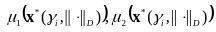
\includegraphics[width=0.8\textwidth]{assets/260}
	\caption*{}
\end{figure}талаптарын
орындай отырып,

− интегрленген критерийдің \begin{figure}[H]
	\centering
	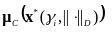
\includegraphics[width=0.8\textwidth]{assets/261}
	\caption*{}
\end{figure}
максималды мәнін қамтамасыз ететін

− тұрақтандыру колоннасының кіріс, режимдік параметрлері векторы
\begin{figure}[H]
	\centering
	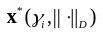
\includegraphics[width=0.8\textwidth]{assets/262}
	\caption*{}
\end{figure}шығарылады.

\emph{Алынған негізгі нәтижелерді талқылау}. Ұсынылып, сипатталған
эвристикалық айқынсыздықта шешім қабылдау алгоритмі Парето оптималдық
принципін критерийлерге, ал айқын емес шектеулерге идеалды нүкте
оптималдық принциптерін айқынсыздыққа бейімдеуге негізделген. Айқын емес
есептерді шешудің бұл эвристикалық тәсілдемесінің, бастапқы айқын емес
есепті \emph{α} деңгейлі жиындар арқылы айқын есептер жиынына
айналдырып, дәстүрлі айқын тәсілдер арқылыы шешуге негізделген белгілі
тәсілдемесінен артықшылығы, эвричстикалық тәсілдемеде бастапқы айқын
емес есеп айқынсыздықта формализацияланып, шешіледі.

Идеясы қысқаша сипатталған айқын емес есептерді шешу тәсілдемесінде
бастапқы айқын емес есепті айқын есептерге түрлендіру процесінде
жинақталған айқын емес ақпараттардың, яғни ШҚТ, эксперттердің
тәжірибесі, білімі және түйсігігің \emph{α} деңгейлдеріндегіден басқа,
айтарлықтай бөлігі қолданылмай қалады. Ал бұл айқынсыздықта құрылған
модельдің адекваатығы мен қабылданған шешімдердің тиімділіген
төмендетеді. \emph{α} деңгейлдері сандарын арттыру арқылы модель
адекваттығы мен шешім тиімдігін арттыру алынған айқын есептердің санын
күрт арттыратындықтан практикалық тұрғыдан тиімсіз болады.

Ұсынылған эвристикалық тәсілдемеде айқынсыздық айқын емес жиындар
теориясының математикалық аппараты арқылды формализациялану және есепті
шешу барысында ШҚТ білім, тәжірибесі мен түйсігі болып табылатын айқын
емес ақпараттарды максималды қолдану есебінен жоғары адекватты модель
мен өте тиімді шешшімдер қабылдауға мүмкіндік береді.

Зерттеу нысанын саралау нәтижесінде осы жұмыста таңдалған Парето
оптималдық принципін критерийлдерге, ал идеалдыв нүкте оптималдық
принципін айқын емес шектеулерге қолдануға қажетті ақпараттардың
қолжетімдігі анықталды. Яғни әзірленіп, сипатталған ПО+ИН алгоритмі
Парето оптималдық, және идеалды нүкте оптимизациялау принциптерін
қолдануға қажетті болатын ШҚТ көмегімен локалды критерийлердің салмақ
коэффициенттері ($\gamma_1=0.8,\gamma_2=0.2$) және айқын емес
шектеулердің орындалу деңгейінің мәні
($\mu_r^1=1,\mu_r^2=1,$ тиістілік функция нормалды
болғандықтан) белгілі. Таңдалған иоптималдықө принциптерін жүзеге
асыруға қажетті шарттар мен ақпараттар болғандықтан қойылған айқын емес
шешім қабылдау есебі айқын емес жиындар мен эксперттік бағалау тәсілдері
негізінде тиімді шешіледі. Яғни ұсынылған эвристикалық тәсіл
критерийлердің салмақ коэффициенттерін анықтау, олардың саны
$5\pm2$ аспағанда және вйқын емес
шектеулердің орындалуының идеалды деңгейі белгілі немесе оның анықталуы
мүмкін болғанда тиімді жүзеге асады.

Келтірілген эвристикалық тәсілдеменің идеясы негізінде таңдалған Парето
оптималдық пен идеалды нүкте оптимизациялау принциптерін қолдануға
қажетті ақпараттар қолжетімсыз, шарттар орындалмаған жағдайда басқа
қолдануға болатын оптималдық принциптері мен олардың түрлі
комбинацияларын қолдануға болады.

Ұсынылған айқын емес есепті айқын есептерге түрлендірмей-ақ,
айқынсыздықта математикалық қойылымын тұжырымдап, оны айқынсыздықта
түрлі оңтайландыру принциптерін модификациялау, комбинациялау негізінде
айқынсыздықпен сипатталатын ШҚТ тәжірибесі, білімі мен шығармашылық
мүмкіндіктерін қолдануға негізделген эвсристикалық тәсілдеменің
жаңашылдығы мен тиімділігін қарастырайық.

Жоғарыда ұсынылып, сипатталған айқынсыздықта тиімді шешім қабылдацу
тәсілдемесі жинақталған және қолжетімді айқынсыздықпен сипатталатын ШҚТ,
эксперттер тәжірибесі, білімі мен түйсігін, олардың шығармашылық
мүмкіндіктерін есепті айқынсыздықта шешу процесінде толықтай қолдануға
мүмкіндік береді. Сәйкесінше айқынсыздықпен сипатталатын көптеген
өндірістік нысандарды модельдеу, олардың жұмыс режимдерін оңтайландыру
есетерін адекватты, тиімді шешімдерін алуға болады. Сонымен қатар
ұсынылған эвсристикалық тәсілдемеде өндірістегі туындаған түрлі
жағдайларға, өндірістік жоспар мен талаптарға, өндірілетін өнімге деген
нарықтағы сұраныс пен талаптарға және ШҚТ басымқыларына байланысты түрлі
параметрлерді өзгерте отырып, ШҚТ ең тиімді шешімді таңдай алады.

Егер критерийлерге талдалған Парето оптималдық пинципін, ал айқын емес
шектеулерге идеалды нүкте принциптерін қолдануға қажетті ақпараттар мен
шарттар болмаса, онда ұсынылған эвристикалық тәсілдеменің идеясына
сәйкес басқа оптималдық принциптері мен комбинациясын айқынсыздыққа
модификациялау арқылы қолдануға болады. Бұл кезде таңдалған оптималдық
принциптерін айқынсыздыққа модификациялау айқын емес параметрлердің
тиістілік функциясын құрып, формализациялау арқылы жүзеге асырылады.

Сонымен таңдалған оптималдық принциптерін қолдануға қажетті ақпараттар
қол жетімсіз болса, ұсынылған айқынсыздықта тиімді шешімдер жиынында
қайшылықта болатын көпкритерийлі оңтайландыру, яғни шешім қабылдау
есебін шешудің эвристикалық тәсілдемесіне сәйкес, туындаған жағдайды
қолдануға ыңғайлы басқа оптитмалдық принцимптері мен олардың
комбинацияларын айқынсыздыққа модификациялау қажет. Егер жоғарыда
зерттеу нысанының жұмыс режимдерін оңтайландыру үшін ыңғайлы болып
табылған Парето оптималдық пен идеалды нүкте оптималдық принциптері
өндірістік жағдайдың өзгеруіне байланысты тиімсіз болса, онда бас
критерий, максимин, теңдік не басқа критерийлерді таңдау керек. Бұл
кезде басқа оптималдық принциптері оларды айқынсыздыққа модификациялап,
қолдануға қажетті ақпараттар мен жағдайдың болуына байланысты таңдап
алынады.

Мысалы айқынсыздықта бірнеше критерийлердің ішінен ең маңыздысын, яғни
басты критерийді анықтау, ал шектеулердің маңыздылықтары жуықша бірдей
болатын болса, онда басты критерий мен теңдік принциптері комбинациясын
модификациялау арқылы оңтайландыру есебін тұжырымдап эвсристикалық
тәсілдеме көмегімен тиімді шешуго болады. Мұндай эвристикалық шешім
қабылдау тәсілі модификацияланған басты критерий (критерийлерге) мен
теңдік принциптерінің (шектеулерге) қолдануға негізделетін болады. Ал
бұл тәсілдеме де белгілі бір себептермен тиімсіз болса, айқынсыздықта
шешім қабылдау есебін тиімді шешу үшін ұсынылған эвртстикалық
тәсілдеменің идеясы негізінде қажетті ақпараттар мен шарттар болатын
басқа оптималдық принциптері мен олардың комбинациясын қолдануға болады.

Айтылғандарды тұжырымлай келе, түрлі өндірістік жағдайлар мен қолжетімді
ақпараттар сипатына байланысты әр түрлі оптималдық принциптерін
модификациялап, олардың түрлі комбинацияларын қолдануға болады. Яғни
ұсынылған айқынсыздықта көпкритерийлі оңтайландыру есебі қойылымын түрлі
оптималдық принциптерін модификациялау арқылы оны математикалық
тұжырымдау және сиатталған эвристикалық жолмен тиімді шешу тәсілдемесі
айтарлықтай әмбебап болып табылады. Айқынсыздықта шешім қабылдау
есептерін шешудің эвристикалық тәсілдемесі шешім қабылдау теориясы мен
тәсілдерін дамытуда және пратикада көптеп кездесетін мұндай өндірістік
есептерді тиімді шешу аясын кеңейтуге айтарлықтай үлес қосады.

{\bfseries Қорытынды.} МБӨ қондырғысында тұрақты бензин өндіру процесін
айқынсыздықта оның модельдері негізінде тиімді оңтайландыру эвристикалық
тәсілдемесі әзірленіп, сипатталған. Ұсынылған айқынсыздыққа өндірісте
туындаған жағдайлар мен қолжетімді ақпараттар сипатына байланысты түрлі
оптималдық принциптері мен олардың комбинацияларын модификациялауға
негізделген эвристикалық тәсілдеме идеясы түрлі жағдайға бейімделе
алатын әмбебап тәсілдеме болып табылады.

Жұмыстың зерттеу мақсаты ретінде тұжырымдалған МБӨ қондырғысының
тұрақтандыру колоннасынан тұрақты бензин өндіру процесін айқынсыздықта
модельдерін құрылып, құрылған модельдер негізінде тұрақтандыру
колоннаның жұмыс режимдерін оңтайландыру эвристикалық тәсілі әзірленді.
Яғни зерттеу мақсатты толықтай қол жеткізіліп, орындалды.

Тұжырымдалған мақсаттың орындалуын қамтамасыз ететін, зетртеу міндеттері
де толықтай шешілім келесі зерттеу нәтижелері алынған:

− зерттеу нысаны ретінде алынған МБӨ қондырғысының тұрақтандыру
колоннасы мысалында оңтайландыру критериийлері болып табылатын кей
параметрлері айқын емес ақпараттармен сипатталатын күрделі технологиялық
нысандардың айқынсыздықта модельдерін түрлі қолжетімді ақпараттар
негізінде құру тәсілдемесі ұсынылған. Бұл тәсілдеме негізінде
өндірілетін МБӨ қогндырғысының мақсаттық өнімі − тұрақты бензиннің
көлемін қолжетімді эксперименталдық-статистикалық деректер, ал айқын
емес сапа көрсеткіштерін ШҚТ, эксперт-мамандар тәжірибесі, білімі
негізінде анықтайтын модельдер құрылды. Құрылған модельдердің құрамы
регрессорларды тізбектей қосу тәмсілдемесі, ал белгісіз параметрлері
(регрессиялық коэффициенттері) модификацияланған ең кіші квадраттар
тәсілі негізінде MatLab жүйесін пайдаланып идентификацияланған.

− Парето оптималдық максимин оптималдық принциптерін айқынсыздыққа
модификациялау арқылы айқынсыздықта тұрақтандыру колоннасының жұмыс
режимдерін векторлық оңтайландыру бойыншща тиімді шешім қабылдау есебі
формализацияланып, математикалық тұжырымдалған. Математикалық қойылымы
алынған айқынсыздықта шешім қабылдау есебін айқын емес ортада тиімді
шешу үшін таңдалған оптималдық принциптерінің модификациясына
негізделген эвсритикалық алгоритм ұсынылып, оның негізгі қадамдары
сипатталған.

− Алынған негізгі нәтижелер талқылып, айқынсыздықта шешім қабылдаудың
ұсынылған эвристикалық тәсілдемесінен белгілі, бастапқы айқын емес
есептепті айқын есептер жиынына түрлендірігу арқылы шешуге негізделген
тәсілдемесінен айырмашалығы мен артықшылықтар негізделген. Ұсынылған
эвристикалық шешім қабылдау тәсілдемесінде де бастапқы айқын емес есеп
айқын есептерге түрлендірілмей-ақ айқынсыздықта қойылып, айқынсыздықта
шешіледі. Яғни мұндай эвристикалық тәсілдеме ақпарат тапшылығы мен
айқынсыздығы жағдайында өте маңызды, мағыналы болып табылдатын
тәжірибелі ШҚТ, эксперт-мамандар білімі, тәжірибесі мен интуициясы
түріндегі айқын емес ақпараттарды толықтай қолдану есебінен құрылған
модельдердің жоғары адекваттығы мен қабвлданған шешімдердің жоғары
тиімділігін қамтамасыз ете алады.

Авторлардың алдағы зерттеулерінде осы жұмыста алынған нәтижелер
негізінде зерттеу нысанын айқынсыздықта компьютерлік модельдеу және оның
жұмыс режимдекрін айқын емес ортада оңтайландыру бойынша ШҚТ-ға тиімді
шешімді оперативті қабылдауға қолдау көрсететін интеллектуалдандырылған
шешім қабылдауды қолдау жүйесін {[}22{]} әзірлеу жоспарланған.

\emph{{\bfseries Қаржыландыру.}} ~\emph{Зерттеу Х. Досмухамедов атындағы
Атырау университетінің қаржыландырған (грант «Мұнай өңдеу өһндірісі
технологиялық кешендерінің жұмыс режимдерін оптимизациялау ишешім
қабылдауды қолдау нтеллектуды жүйелері − Интеллектуальные системы
принятия решений для оптимизации режимов работы технологических
комплексов нефтеперерабатывающего производства}»\emph{).}


\begin{center}
	{\bfseries Литература}
	\end{center}

\begin{noparindent}

1. Сериков Т.П. Современные технологии и процессы переработки нефти и
газа. - Алматы: Гылым, 2018. 357 с.

2. Beltramini J.N., Lu G.Q. Processing of Primary and Secondary Fuels:
Perspective on Petroleum Refining // Energy Storage Systems. 2020. Vol.
2(1). −P.1−28.

http://www.eolss.net/Eolss-sampleAllChapter.aspx

3. Ахметов С.А. Технология и оборудование процессов переработки нефти и
газа. - СПб.: Недра, 2006. - 871 с. ISBN 5-94089-074-1

4. Кафаров, В. В. Системный анализ процессов химической технологии :
основы стратегии: монография / В. В. Кафаров, И. Н. Дорохов.- Москва :
Изд-во Юрайт, 2018. - 499 с. ISBN 978-5-534-06991-4.

5. Chen Y., He L., Li J., Zhang S. Multi-criteria design of
shale-gas-water supply chains and production systems towards optimal
life cycle economics and greenhouse gas emissions under uncertainty //
Computers \& chemical engineering. 2018. -Vol. 109. -P. 216--235.
https://doi.org/10.1016/j.compchemeng.2017.11.014

6. Zimmermann H.-J. Fuzzy Set Theory -- and Its Applications. Springer
Science+Business Media //LLC. Fifth Edition. -2018. -525 p. ISBN:
978-94-010-3870-6

7. Orazbayev B.B., Orazbayeva K.N., Utenova B.E. Development of
Mathematical Models and Modeling of Chemical Engineering Systems under
Uncertainty // Theoretical Foundations of Chemical Engineering. 2014.
--Vol. 48. № 4. -- P. 138--147. DOI:10.1134/S0040579514020092

8. Orazbayev B., Ospanov Ye., Makhatova V., Salybek L., Abdugulova Z,
Suleimenova S,.Orazbayeva K. Methods of Fuzzy Multi-Criteria Decision
Making for Controlling the Operating Modes of the Stabilization Column
of the Primary Oil-Refining Unit // Mathematic\emph{s.} 2023. Vol. 11,
2820. −Р. 1--20. https://doi.org/10.3390/ math11132820

9. Сулейменов E.Б., Tулеуов Ж.Н. Технологический регламент установки
первичной переработки нефти ЭЛОУ-АТ-2. -Атырау, изд. АУНГ, 2019. -112 с.

10. ГОСТ 2177 (ИСО 3405-88) − Нефтепродукты. Способы определения
качества и фракционного состава. --Минск, 2002. -23 с.

11. Бойко, И.А. Математические модели технологических систем в условиях
неопределенности // Молодой ученый. 2019. № 6(53). -С. 30-33. URL:
https://moluch.ru/archive/53/7208/ (дата обращения: 24.06.2024).

12. Зайченко Ю.П. Исследование операций: нечеткая оптимизация. --Киев:
Изд-во Выща школа, 1991. -193 с. ISBN: 5-11-002276-3

13. Волин Ю.М., Островский Г.М. Многокритериальная оптимизация
технологических процессов в~условиях неопределенности // Автоматика и
телемеханика. -- 2007. -- Т. 53. -- №~3. -- С. 165--178.

14. Оразбаев Б.Б., Асанова Б.У., Молдашева Ж.Ж., Шуйтенов Г.Ж.,
Дюсембина Э.М. Түрлі сипаттағы қол жетімді ақпараттар негізінде баяу
кокстеу қондырғысының өзара байланысқан технологиялық агрегаттары
модельдерін құру әдістемесі // News of the National Academy of Sciences
of the Republic of Kazakhstan, Physico-Mathematical series. 2023. Vol.
3. № 347. -С.28--43 https://doi.org/10.32014/2023.2518-1726.202

15. Салыбек Л.Т., Оразбаева К.Н., Махатова В.Е., Курмангазиева Л.Т.,
Утенова Б.Е. Мұнайды алғашқы өңдеу қондырғысы атмосфералық блогының
модельдерін түрлі сипаттағы қолжетімді ақпарат негізінде құру // News of
the National Academy of Sciences of the Republic of Kazakhstan,
Physico-Mathematical series. -2023. - Vol. 2. -№ 350. -С.285--296.

https://doi.org/10.32014/2024.2518-1726.283

16. Huang H.Z., He L. New Approaches to System Analysis and Design: A
Review. In: Misra, K.B. (eds) Handbook of Performability Engineering.
-Springer, London. 2019. -P. 477--498.
https://doi.org/10.1007/978-1-84800-131-2\_31

17. Карманов Ф.И. Острейковский В.А. Статистические методы обработки
экспериментальных данных с использованием пакета MathCad, -М.: Радио и
связь, 2019.\\
-187 с. ISBN: 978-5-905554-96-4.

18. Douglas A.M. and Danny A.M. Statistical Methods in Experimental
Pathology: A Review and Primer. The American Journal of Pathology.
-2021. -Vol. 191(5). --P. 784--794.
https://doi.org/10.1016/j.ajpath.2021.02.009.

19. Zhao Zh.W., Wang D.H. Statistical inference for generalized random
coefficient autoregressive model // Mathematical and Computer Modelling.
-- 2018. - Vol.56(3). -Р.152-166.

20. Jorgensen M. A Review of Studies on Expert Estimation of Software
Development Effort. Journal of Systems and Software. -2019{\bfseries .}
-Vol.70. -Р.37-60. DOI:10.1016/S0164-1212(02)00156-5

21. Рыжов А.П. Теория нечетких множеств и ее приложения. -Москва: МГУ.
2-е издание. 2021. -285 с. ISBN: 978-3-540-70777-6.

21. Fuzzy Logic Toolbox. Available online: http://www.matlab.ru (доступ
25 августа 2024 г.).

22. Hamilton S.H., Jakeman A.J., Norton J.P. Artificial Intelligence
techniques: An introduction to their use for modelling environmental
systems // Mathematics and Computers in Simulation.-2018. -Vol. 78(2).
-P. 379--400. https://doi.org/10.1016/j.matcom.2008.01.028

\end{noparindent}

\begin{center}
	{\bfseries References}
	\end{center}

\begin{noparindent}

1. Serikov T.P. Sovremennye tehnologii i processy pererabotki nefti i
gaza. - Almaty: Gylym, 2018. 357 s. {[}in Russian{]}

2. Beltramini J.N., Lu G.Q. Processing of Primary and Secondary Fuels:
Perspective on Petroleum Refining // Energy Storage Systems. 2020. Vol.
2(1). P.128. http://www.eolss.net/Eolss-sampleAllChapter.aspx

3. Ahmetov S.A. Tehnologija i oborudovanie processov pererabotki nefti i
gaza. - SPb.: Nedra, 2006. - 871 s. ISBN 5-94089-074-1 {[}in Russian{]}

4. Kafarov, V. V. Sistemnyj analiz processov himicheskoj tehnologii :
osnovy strategii: monografija / V. V. Kafarov, I. N. Dorohov.- Moskva :
Izd-vo Jurajt, 2018. - 499 s. ISBN 978-5-534-06991-4. {[}in Russian{]}

5. Chen Y., He L., Li J., Zhang S. Multi-criteria design of
shale-gas-water supply chains and production systems towards optimal
life cycle economics and greenhouse gas emissions under uncertainty //
Computers \& chemical engineering. 2018. -Vol. 109. -P. 216--235.
https://doi.org/10.1016/j.compchemeng.2017.11.014

6. Zimmermann H.-J. Fuzzy Set Theory -- and Its Applications. Springer
Science+Business Media //LLC. Fifth Edition. -2018. -525 p. ISBN:
978-94-010-3870-6

7. Orazbayev B.B., Orazbayeva K.N., Utenova B.E. Development of
Mathematical Models and Modeling of Chemical Engineering Systems under
Uncertainty // Theoretical Foundations of Chemical Engineering. 2014.
--Vol. 48. № 4. -- P. 138--147. DOI:10.1134/S0040579514020092

8. Orazbayev B., Ospanov Ye., Makhatova V., Salybek L., Abdugulova Z,
Suleimenova S,.Orazbayeva K. Methods of Fuzzy Multi-Criteria Decision
Making for Controlling the Operating Modes of the Stabilization Column
of the Primary Oil-Refining Unit // Mathematics. 2023. Vol. 11, 2820.
R. 1--20. https://doi.org/10.3390/ math11132820

9. Sulejmenov E.B., Tuleuov Zh.N. Tehnologicheskij reglament ustanovki
pervichnoj pererabotki nefti JeLOU-AT-2. -Atyrau, izd. AUNG, 2019. -112
s. {[}in Russian{]}

10. GOST 2177 (ISO 3405-88) Nefteprodukty. Sposoby opredelenija
kachestva i frakcionnogo sostava. --Minsk, 2002. -23 s. {[}in Russian{]}

11. Bojko, I.A. Matematicheskie modeli tehnologicheskih sistem v
uslovijah neopredelennosti // Molodoj uchenyj. 2019. № 6(53). -S. 30-33.
URL: https://moluch.ru/archive/53/7208/ (data obrashhenija: 24.06.2024).
{[}in Russian{]}

12. Zajchenko Ju.P. Issledovanie operacij: nechetkaja optimizacija.
--Kiev: Izd-vo Vyshha shkola, 1991. -193 s. ISBN: 5-11-002276-3 {[}in
Russian{]}

13. Volin Ju.M., Ostrovskij G.M. Mnogokriterial\textquotesingle naja
optimizacija tehnologicheskih processov v uslovijah neopredelennosti //
Avtomatika i telemehanika. -- 2007. -- T. 53. -- № 3. -- S. 165--178.
{[}in Russian{]}

14. Orazbaev B.B., Asanova B.U., Moldasheva Zh.Zh., Shujtenov G.Zh.,
Djusembina Je.M. Túrli sipattaǵy qol zhetimdi aqparattar negizinde bajau
koksteu qondyrǵysynyń ózara bajlanysqan tehnologijalyq agregattary
model\textquotesingle derin qugı ádistemesi // News of the National
Academy of Sciences of the Republic of Kazakhstan, Physico-Mathematical
series. 2023. Vol. 3. № 347. -S.28-43
https://doi.org/10.32014/2023.2518-1726.202 {[}in Kazakh{]}

15. Salybek L.T., Orazbaeva K.N., Mahatova V. E., Kurmangazieva L.T.,
Utenova B.E. Munajdy alǵashqy óńdeu qondyrǵysy atmosferalyq blogynyń
model\textquotesingle derin túrli sipattaǵy qolzhetimdi aqparat
negizinde qugı // News of the National Academy of Sciences of the
Republic of Kazakhstan, Physico-Mathematical series. -2023. - Vol. 2. -№
350. -S.285-296. https://doi.org/10.32014/2024.2518-1726.283 {[}in
Kazakh{]}

16. Huang H.Z., He L. New Approaches to System Analysis and Design: A
Review. In: Misra, K.B. (eds) Handbook of Performability Engineering.
-Springer, London. 2019. -P. 477--498.
https://doi.org/10.1007/978-1-84800-131-2\_31

17. Karmanov F.I. Ostrejkovskij V.A. Statisticheskie metody obrabotki
jeksperimental\textquotesingle nyh dannyh s
ispol\textquotesingle zovaniem paketa MathCad, -M.: Radio i
svjaz\textquotesingle, 2019. -187 s. ISBN: 978-5-905554-96-4. {[}in
Russian{]}

18. Douglas A.M. and Danny A.M. Statistical Methods in Experimental
Pathology: A Review and Primer. The American Journal of Pathology.
-2021. -Vol. 191(5). --P. 784--794.
https://doi.org/10.1016/j.ajpath.2021.02.009.

19. Zhao Zh.W., Wang D.H. Statistical inference for generalized random
coefficient autoregressive model // Mathematical and Computer Modelling.
-- 2018. - Vol.56(3). -R.152-166.

20. Jorgensen M. A Review of Studies on Expert Estimation of Software
Development Effort. Journal of Systems and Software. -2019. -Vol.70.
-R.37-60. DOI:10.1016/S0164-1212(02)00156-5

21. Ryzhov A.P. Teorija nechetkih mnozhestv i ee prilozhenija. -Moskva:
MGU. 2-e izdanie. 2021. -285 s. ISBN: 978-3-540-70777-6. {[}in
Russian{]}

21. Fuzzy Logic Toolbox. Available online: http://www.matlab.ru (dostup
25 avgusta 2024 g.).

22. Hamilton S.H., Jakeman A.J., Norton J.P. Artificial Intelligence
techniques: An introduction to their use for modelling environmental
systems // Mathematics and Computers in Simulation.-2018. -Vol. 78(2).
-P. 379--400. https://doi.org/10.1016/j.matcom.2008.01.028
\end{noparindent}

\emph{{\bfseries Авторлар жайында мәліметтер:}}
\begin{noparindent}

Оразбаев Б.Б. -- техника ғылымдарының докторы, Қазақстан Республикасы
Инженерлік академиясының академигі, Жүйелік талдау және басқару
кафедрасының профессоры, Л.Н.Гумилев атындағы Еуразия ұлттық
университеті, Астана қ., Қазақстан,е-mail: batyr\_o@mail.ru;

Салыбек Л.Т. − М. Әуезов атындағы Оңтүстік Қазақстан университеті
докторанты, Қазақстан, е-mail: lyaklai.36972@mail.ru;

Курмангазиева Л.Т. -- Х.Досмухамедов атындағы Атьрау университеті,
техника ғылымдарының кандидаты, Программалық инженерия кафедрасының
профессоры, Атырау қ., Қазақстан, е-mail: kuzhuhanova-zhad@mail.ru;

Терехов В.И. − Бауман атындағы Мәскеу мемлекеттік техникалық
университетіі, техника ғылымдарының кандидаты, доцент, Мәскей қ., Ресей
Федерациясы, е-mail: terekchow@bmstu.ru;

Утегова Б.П. -- С. Утебаев атындағы Атырау мұнай және газ университеті,
техника ғылымдарының кандидаты, Ақпараттық технологиялар факультетінің
қауымдасқан профессоры, Атырау қ., Қазақстан, е-mail:
balbupe\_u\_e@mail.ru;

Махатова В.Е. -- Х.Досмухамедов атындағы Атырау университеті, техника
ғылымдарының кандидаты, Программалық инженерия кафедрасының профессоры,
Атырау қ., Қазақстан, е-mail: mahve@mail.ru;

Өтебаева А.С. -- Х.Досмухамедов атындағы Атырау университеті, магистр,
Программалық инженерия кафедрасының ағы оқытушысы, Атырау қ., Қазақстан,
е-mail: aotebayevas@mail.ru
\end{noparindent}

\emph{{\bfseries Information about the authors}}
\begin{noparindent}

Orazbayev B.B. \emph{--} doctor of technical sciences, academician of
the Engineering academy of the republic of Kazakhstan, professor of the
department of System analysis and Control, L.N. Gumilyov Eurasian
National University, Astana, Kazakhstan, е-mail: batyr\_o@mail.ru;

Salybek L.Т. -- doctoral student, M. Auezov South Kazakhstan University,
Shymkent, Kazakhstan, е-mail: lyaklai.36972@mail.ru;

Курмангазиева Л.Т. -- Kh. Dosmukhamedov Atyrau University, Candidate of
Technical Sciences, Professor of the Department of Software Engineering,
Аtyrau. Kazakhstan, е-mail: kuzhuhanova-zhad@mail.ru;

Terekhov V.I. -- Bauman Moscow State Technical University, candidate of
technical sciences, associate professor, Moscow, Russian
Federation,е-mail: terekchow@bmstu.ru;

Утенова Б.П. -- Атырауский университет нефти и газа имени С. Утебаева,
кандидат технических наук, доцент факультета информационных технологий,
Атырау, Казахстан, е-mail: balbupe\_u\_e@mail.ru;

Маkhatova V.E -- Kh. Dosmukhamedov Atyrau University, Candidate of
Technical Sciences, Professor of the Department of Software Engineering,
Аtyrau. Kazakhstan, е-mail: mahve@mail.ru;

Otebayeva A.A.-- Kh. Dosmukhamedov Atyrau University, Master, Senior
Lecturer, Department of Software Engineering, Аtyrau. Kazakhstan,
е-\/-mail: aotebayevas@mail.ru
\end{noparindent}
